% ----------------------------------------------------------

\chapter{METODOLOGIA}

% ----------------------------------------------------------



\begin{figure}[htbp]
    \centering
    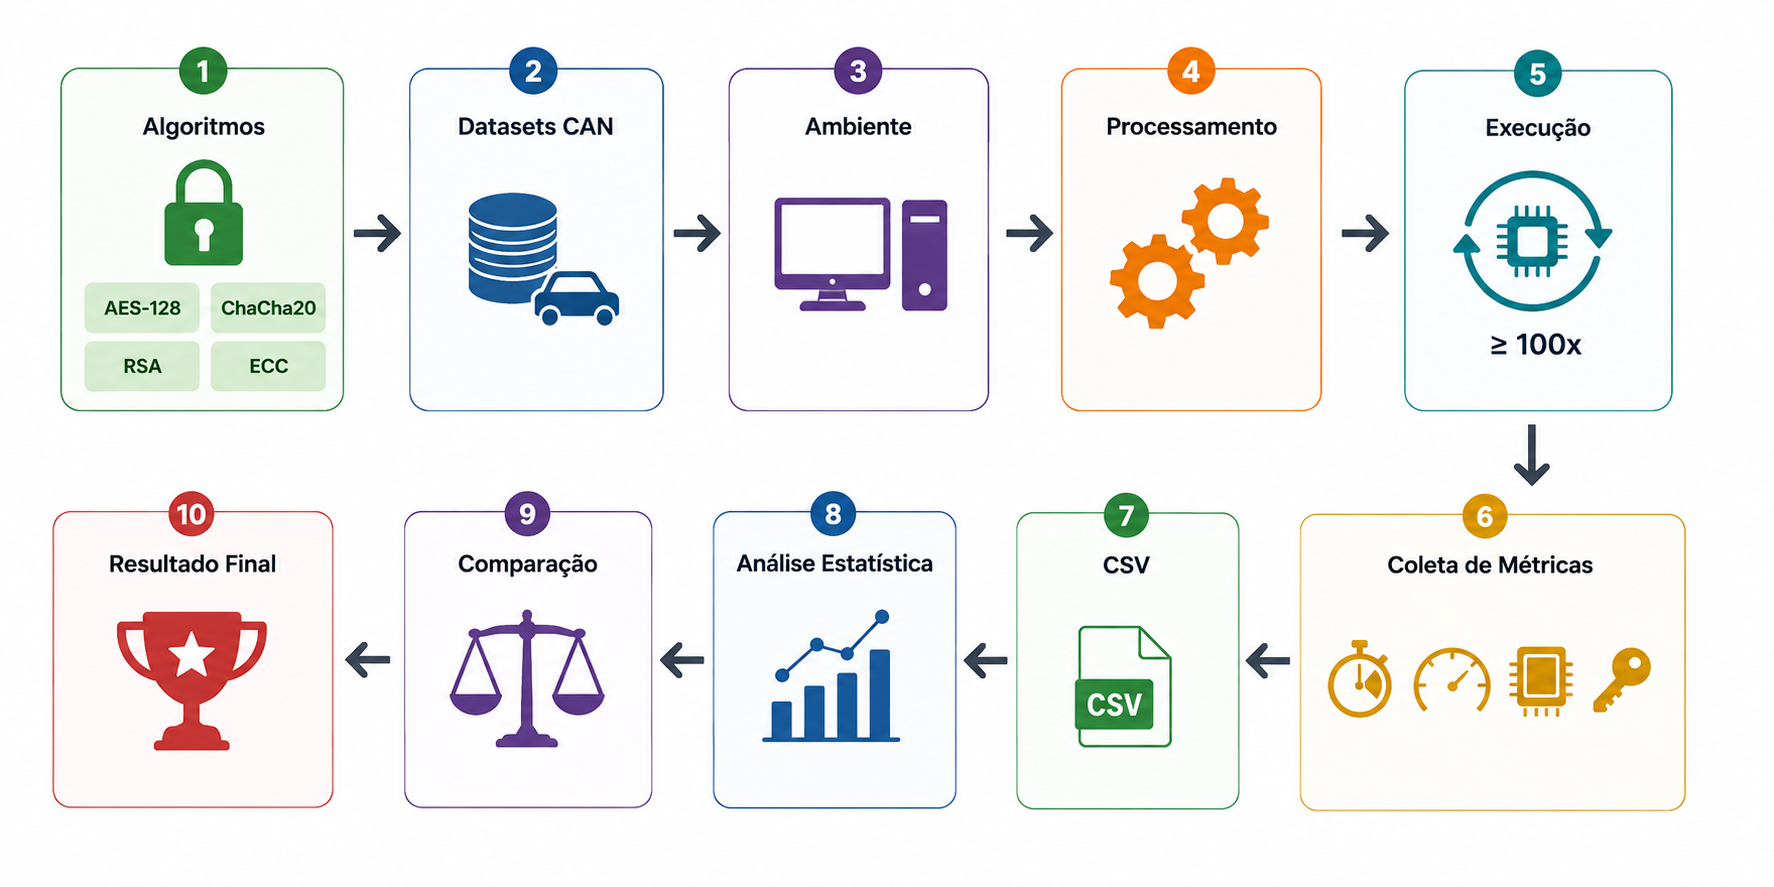
\includegraphics[width=1.0\textwidth]{images/metodologia.jpg}
    \caption{Workflow da Metodologia do Trabalho}
    \label{fig:metodologia}
\end{figure}



Este trabalho possui natureza aplicada, abordagem quantitativa e caráter experimental. O objetivo da pesquisa é comparar o desempenho de diferentes tipos de algoritmos criptográficos no contexto de mensagens de barramento CAN, buscando identificar quais abordagens apresentam maior adequação a sistemas embarcados automotivos sujeitos a restrições de tempo real.



A pesquisa é classificada como quantitativa porque sua análise é baseada na coleta e interpretação de métricas numéricas obtidas por meio da execução controlada dos algoritmos estudados. Também é caracterizada como experimental, uma vez que envolve a realização de testes em ambiente controlado, permitindo a observação direta do comportamento dos algoritmos sob condições previamente definidas.



A metodologia adotada utiliza técnicas de benchmarking para avaliação de desempenho. Essa abordagem é amplamente empregada na análise de sistemas computacionais e permite comparar diferentes soluções de forma objetiva por meio da mensuração de métricas relacionadas ao custo computacional. Neste trabalho, o benchmarking é utilizado para avaliar o impacto introduzido por diferentes algoritmos criptográficos sobre dados que representam mensagens potencialmente transmitidas em um barramento CAN.

\section{Algoritmos Criptográficos Avaliados}

Foram selecionados quatro mecanismos criptográficos com características e funções distintas. Para a cifragem simétrica, foram considerados AES-128 no modo CTR e ChaCha20, que operam diretamente sobre os dados de entrada. Para a avaliação de operações assimétricas e híbridas, foram considerados RSA-2048 com OAEP e uma construção inspirada no \textit{Elliptic Curve Integrated Encryption Scheme} (ECIES), baseada na curva P-256.

O AES-128-CTR representa o uso de uma cifra de bloco em modo de operação que dispensa preenchimento, enquanto o ChaCha20 representa uma cifra de fluxo voltada à cifragem eficiente em software. O RSA-2048-OAEP foi incluído para caracterizar o custo de uma operação de cifragem assimétrica. O ECIES-P256, por sua vez, foi selecionado para representar uma construção híbrida que emprega criptografia de curvas elípticas (ECC), por meio do ECDH, para obter material de chave posteriormente utilizado em cifragem simétrica.

\section{Parâmetros das Implementações Criptográficas}

Os mecanismos avaliados foram definidos com parâmetros criptográficos específicos, de modo a identificar as operações efetivamente executadas em cada ambiente experimental. O AES-128-CTR utiliza uma chave simétrica de 128 bits e opera em modo contador, sem necessidade de preenchimento dos dados. O ChaCha20 utiliza uma chave simétrica de 256 bits e realiza a cifragem por meio da combinação dos dados de entrada com um fluxo pseudoaleatório.

O RSA-2048-OAEP utiliza um par de chaves RSA de 2048 bits e o esquema de preenchimento OAEP para a operação de cifragem assimétrica. A função de resumo empregada no OAEP deve ser identificada conforme a configuração efetiva da implementação.

A construção híbrida experimental denominada ECIES-P256 utiliza operações ECDH sobre a curva secp256r1, seguida da aplicação de SHA-256 ao segredo compartilhado e do emprego de AES-128-GCM para a cifragem dos dados. Essa construção não representa uma implementação integral de um perfil ECIES padronizado, sendo utilizada exclusivamente para avaliar o custo computacional das operações implementadas.

Os parâmetros de inicialização, o gerenciamento das chaves e a delimitação das regiões temporizadas devem ser interpretados conforme a implementação efetivamente utilizada em cada ambiente. As diferenças entre OpenSSL e mbedTLS são consideradas na análise, não sendo presumida equivalência de desempenho entre as bibliotecas.

\section{Critérios de Comparabilidade entre os Mecanismos}

A seleção de mecanismos de diferentes categorias exige distinguir a função criptográfica executada em cada caso. AES-128-CTR e ChaCha20 realizam cifragem simétrica direta e, quando aplicados à mesma carga útil sob condições de medição equivalentes, permitem uma comparação mais direta de latência e throughput. RSA-2048-OAEP e ECIES-P256, entretanto, envolvem operações assimétricas ou híbridas, com etapas, formatos de saída e custos distintos. Consequentemente, seus tempos não devem ser interpretados como medidas de uma mesma operação criptográfica.

Neste trabalho, as métricas de todos os mecanismos são apresentadas para caracterizar seus custos computacionais no ambiente de teste, mas as conclusões são organizadas conforme a função desempenhada. A comparação principal de cifragem por mensagem ocorre entre AES-128-CTR e ChaCha20. Para RSA-2048-OAEP e ECIES-P256, a análise considera separadamente o custo das operações implementadas, incluindo geração ou estabelecimento de chaves quando mensurados, e sua pertinência a etapas pontuais de uma possível arquitetura de segurança veicular.

A padronização do ambiente, da entrada e dos instrumentos de medição reduz fatores externos de variação, mas não torna funcionalmente equivalentes os quatro mecanismos. Além disso, o tempo de geração de chaves não deve ser confundido com o tempo de cifragem por mensagem nem somado a ele sem especificar a frequência com que essa etapa ocorreria. Assim, os resultados permitem discutir adequação computacional e possíveis funções complementares, sem afirmar que o mecanismo com menor latência isolada oferece necessariamente a melhor solução de segurança para o barramento CAN.

\section{Ambiente Experimental}

A avaliação dos algoritmos criptográficos foi realizada em um ambiente experimental controlado, com o objetivo de garantir a consistência e a reprodutibilidade das medições de desempenho. A utilização de um ambiente controlado permite minimizar a interferência de variáveis externas, assegurando que os resultados obtidos reflitam predominantemente o comportamento dos algoritmos analisados.

O ambiente experimental foi implementado utilizando a linguagem de programação C, em conjunto com a biblioteca criptográfica OpenSSL. Essa biblioteca foi escolhida por disponibilizar implementações amplamente utilizadas, otimizadas e consolidadas dos algoritmos avaliados, permitindo maior fidelidade na análise de desempenho.

Os experimentos foram executados em um sistema computacional com as seguintes características:


\begin{itemize}

\item Processador AMD Ryzen 5 3600, frequência base de 3,6 GHz e seis núcleos físicos;

\item Memória RAM de 16 GB;

\item Sistema Operacional Windows 11 de 64 bits.

\end{itemize}

A especificação detalhada do hardware utilizado é importante porque o desempenho dos algoritmos criptográficos está diretamente relacionado à capacidade de processamento disponível. Dessa forma, a descrição do ambiente experimental contribui para a reprodutibilidade dos resultados e facilita futuras comparações com outros estudos.

Para garantir a rastreabilidade da configuração computacional, foram considerados o sistema operacional utilizado, a versão da biblioteca OpenSSL e o compilador empregado. Esses parâmetros são relevantes porque diferenças entre versões de bibliotecas, opções de compilação e recursos de aceleração criptográfica podem influenciar os tempos registrados.

No ambiente Windows, a latência foi mensurada por meio das funções QueryPerformanceCounter e QueryPerformanceFrequency, disponibilizadas pela API do sistema operacional. O intervalo de medição foi delimitado pelos registros temporais realizados imediatamente antes e após a região de processamento definida para cada mecanismo criptográfico. A interpretação dos resultados considera as operações incluídas nesse intervalo, distinguindo o tempo de processamento criptográfico das demais etapas do programa.

Os experimentos utilizarão \textit{*datasets*} públicos de tráfego CAN, contendo registros de mensagens capturadas em barramentos automotivos reais ou em ambientes experimentais voltados à pesquisa em segurança veicular. Esses conjuntos de dados serão utilizados como entrada para o programa desenvolvido em linguagem C, permitindo que os algoritmos criptográficos sejam executados sobre mensagens com estrutura semelhante àquelas transmitidas em redes CAN.

Cada registro dos \textit{*datasets*} será tratado como uma representação de mensagem CAN, considerando principalmente os campos relacionados ao identificador da mensagem e ao campo de dados. O conteúdo útil das mensagens será utilizado como entrada para as operações criptográficas, respeitando o objetivo do trabalho, que é avaliar o custo computacional da aplicação dos algoritmos e não interpretar semanticamente o significado de cada mensagem veicular.

Antes da execução dos algoritmos, os dados dos \textit{*datasets*} serão lidos pelo programa desenvolvido em linguagem C a partir dos arquivos disponibilizados pelos conjuntos de dados selecionados. Durante essa etapa, serão extraídas as informações necessárias para representar as mensagens CAN, especialmente os campos relacionados ao identificador da mensagem e ao conteúdo transportado no campo de dados (\textit{*Data Field*}).

Após a leitura, os dados serão convertidos para estruturas internas do programa, permitindo que sejam processados de maneira uniforme por todos os algoritmos avaliados. Dependendo do formato original do \textit{*dataset*}, poderão ser realizadas etapas de pré-processamento, como remoção de informações não utilizadas nos experimentos, padronização da representação dos dados e conversão de valores para formatos compatíveis com as rotinas criptográficas implementadas.

Em seguida, o conteúdo das mensagens será organizado em blocos de dados utilizados como entrada para os algoritmos AES-128-CTR, ChaCha20, RSA-2048-OAEP e ECIES-P256. Essa padronização é necessária para controlar as características dos dados de entrada. Essa padronização não elimina as diferenças funcionais entre as operações simétricas, assimétricas e híbridas, que serão consideradas na análise dos resultados.

A utilização de \textit{*datasets*} públicos contribui para aumentar a representatividade dos experimentos, uma vez que os testes deixam de depender exclusivamente de dados gerados artificialmente. Além disso, o uso de conjuntos de dados disponíveis publicamente favorece a reprodutibilidade da pesquisa, permitindo que outros trabalhos possam repetir ou comparar os resultados obtidos.

Neste trabalho, os \textit{*datasets*} não serão utilizados para classificação de ataques, detecção de intrusão ou análise de comportamento do veículo. Sua função metodológica será fornecer mensagens CAN de referência para que seja possível medir o impacto computacional dos algoritmos criptográficos sobre dados compatíveis com o contexto de aplicação estudado.

Além do ambiente computacional baseado em Windows, foi preparada uma plataforma embarcada ESP32 para a avaliação da latência de processamento criptográfico. Nesse ambiente, os mecanismos AES-128-CTR, ChaCha20, RSA-2048-OAEP e uma construção híbrida experimental baseada em ECIES-P256 foram implementados em linguagem C/C++, utilizando a biblioteca mbedTLS disponibilizada pelo ambiente Arduino.

Os testes na plataforma embarcada foram configurados para utilizar uma entrada fixa de seis bytes, representada pela sequência hexadecimal \texttt{23 A4 19 C8 00 01}. Diferentemente dos experimentos realizados no computador, que utilizam mensagens provenientes de datasets públicos, a entrada fixa permite manter constante o tamanho dos dados durante as medições no ESP32.

A construção híbrida experimental baseada em ECIES-P256 utiliza o protocolo ECDH sobre a curva secp256r1, a função de resumo SHA-256 aplicada ao segredo compartilhado e a cifragem simétrica AES-128-GCM. Essa implementação é utilizada para caracterizar o custo das operações criptográficas executadas, não constituindo uma implementação integral de um perfil ECIES padronizado.

A medição interna da latência foi configurada por meio da função \texttt{esp\_timer\_get\_time()}, que registra os instantes imediatamente anterior e posterior à execução da rotina criptográfica. Paralelamente, o pino GPIO2 é colocado em nível lógico alto antes do início da medição interna e retorna ao nível baixo após seu término, permitindo observar a duração da janela de execução por meio de um osciloscópio.

As chaves criptográficas são preparadas durante a inicialização do programa, enquanto os vetores de inicialização e nonces necessários são gerados antes de cada operação temporizada. O programa permite a seleção individual dos mecanismos pela interface serial e realiza execuções sucessivas, com intervalo configurado de 50 milissegundos após cada teste.

No ESP32, a seleção do mecanismo criptográfico é realizada manualmente pelo monitor serial. Após a seleção, a rotina correspondente é executada sucessivamente até a interrupção do procedimento. Portanto, a quantidade de medições dessa plataforma depende do número de execuções efetivamente registradas, não sendo presumida a realização automática de 100 rodadas.

A preparação inicial das chaves ocorre fora da região temporizada, assim como a preparação dos vetores de inicialização e nonces antes de cada operação. A janela de medição é delimitada pelas chamadas ao temporizador interno, enquanto o pulso gerado no GPIO2 permite observar externamente o intervalo instrumentado. Os resultados devem ser interpretados considerando as operações efetivamente incluídas nessa janela.

As medições internas permitem calcular média, desvio padrão amostral, valores mínimo e máximo. A largura dos pulsos observados no osciloscópio será utilizada como uma medição externa complementar, considerando que o acionamento do GPIO2 introduz um custo adicional de instrumentação. Os resultados dessa etapa serão analisados após a realização das capturas experimentais.


\section{Métricas de Avaliação}

A principal métrica utilizada neste trabalho é a latência de processamento. Essa escolha está diretamente relacionada às características do barramento CAN, que é amplamente empregado em sistemas embarcados de tempo real. Nesses sistemas, atrasos adicionais podem impactar diretamente o comportamento das aplicações e a previsibilidade temporal da comunicação.

A latência representa o tempo necessário para que uma operação criptográfica seja concluída. Quanto menor a latência introduzida pelo algoritmo, menor tende a ser seu impacto sobre o processamento das mensagens. Além da latência, são utilizadas métricas complementares para auxiliar na análise dos resultados.

Neste estudo, a latência é definida operacionalmente como o intervalo de tempo entre o início e o término das operações criptográficas delimitadas nos programas experimentais. Os valores registrados correspondem ao processamento executado pelas implementações avaliadas, não incluindo o tempo de transmissão física, arbitragem ou recepção de quadros no barramento CAN. Para os mecanismos assimétricos e híbridos, a interpretação dos resultados considera as etapas efetivamente incluídas na região temporizada.

O throughput é empregado para representar a quantidade de dados processados por unidade de tempo. Embora o barramento CAN utilize mensagens curtas, essa métrica fornece uma visão geral da eficiência computacional dos algoritmos. O consumo de memória também é analisado, permitindo avaliar a viabilidade de utilização dos algoritmos em sistemas embarcados com recursos limitados.

Para os mecanismos assimétricos e híbridos, é considerado adicionalmente o tempo necessário para geração de chaves, quando essa operação é realizada e medida separadamente. Dessa forma, a comparação entre os mecanismos adota a seguinte hierarquia de avaliação:

\begin{enumerate}
    \item Latência, considerada a métrica principal;
    \item Throughput, utilizado como métrica secundária;
    \item Consumo de memória, utilizado como métrica complementar;
    \item Tempo de geração de chaves, aplicado aos mecanismos assimétricos e híbridos.
\end{enumerate}

Consequentemente, a análise não considera apenas o maior throughput, mas também o custo temporal e computacional das operações avaliadas, respeitando as diferenças funcionais entre os mecanismos criptográficos.

A mensuração do tempo de execução no ambiente Windows foi realizada por meio das funções \texttt{QueryPerformanceCounter} e \texttt{QueryPerformanceFrequency}, disponibilizadas pela API do sistema operacional. Essas funções permitem calcular o intervalo decorrido entre dois instantes registrados durante a execução.

O consumo de memória no ambiente Windows foi obtido por meio da função \texttt{GetProcessMemoryInfo}, pertencente à biblioteca \texttt{psapi}. Essa função permite acessar informações relacionadas ao uso de memória do processo em execução, incluindo memória residente e pico de utilização observado durante os testes.

\section{Procedimento Experimental}

O procedimento experimental será iniciado pela leitura dos \textit{*datasets*} públicos de mensagens CAN. Após a leitura, os registros serão tratados pelo programa desenvolvido em linguagem C, extraindo-se os dados necessários para a execução dos algoritmos criptográficos avaliados.

Em seguida, as mensagens serão submetidas aos algoritmos AES-128-CTR, ChaCha20, RSA-2048-OAEP e ECIES-P256. Para os algoritmos simétricos, serão realizadas operações de cifragem sobre os dados das mensagens. Para os algoritmos assimétricos, além das operações criptográficas correspondentes, será considerado também o tempo de geração de chaves, devido ao impacto dessa etapa no custo computacional dessas técnicas.

Cada algoritmo será executado no mínimo 100 vezes para cada conjunto de dados analisado. A repetição das execuções tem como objetivo reduzir oscilações ocasionais causadas pelo sistema operacional, pela carga momentânea do processador e por variações naturais do ambiente de execução. Dessa forma, os valores analisados não dependerão de uma única medição isolada, mas de um conjunto de execuções capaz de representar melhor o comportamento médio dos algoritmos.

Durante cada execução serão coletadas as métricas de latência, throughput, consumo de memória e, quando aplicável, tempo de geração de chaves. Essas informações serão registradas individualmente pelo programa e exportadas para arquivos no formato CSV, permitindo posterior organização, análise estatística e construção de tabelas e gráficos comparativos.

Após a geração dos arquivos CSV, os resultados serão analisados de forma comparativa. A latência será utilizada como métrica principal, por estar diretamente relacionada aos requisitos temporais do barramento CAN. O throughput e o consumo de memória serão utilizados como métricas complementares, contribuindo para uma avaliação mais ampla da eficiência computacional de cada algoritmo.

Todos os experimentos serão realizados sob as mesmas condições de hardware e software, utilizando o mesmo ambiente experimental, os mesmos critérios de medição e a mesma estrutura de processamento dos dados. Essa padronização busca garantir que as diferenças observadas nos resultados estejam associadas ao comportamento dos algoritmos criptográficos, e não a variações no ambiente de execução.

Os experimentos de desempenho criptográfico não incluem a transmissão física das mensagens cifradas pelo barramento CAN. No ambiente computacional, as operações são realizadas sobre dados carregados em memória, enquanto no ESP32 a avaliação utiliza uma entrada fixa de seis bytes. A bancada física de comunicação CAN, utilizada para demonstração e recepção de mensagens, constitui uma atividade distinta das medições de latência criptográfica e não fornece medidas de desempenho de transmissão de mensagens cifradas.

Essa decisão foi tomada com o objetivo de isolar o custo computacional introduzido pelos algoritmos criptográficos. Em uma rede real, fatores como arbitragem do barramento, carga da rede, latência de transmissão e interação entre múltiplos dispositivos poderiam influenciar os resultados, dificultando a comparação direta entre os algoritmos.

Dessa forma, a metodologia concentra-se especificamente na avaliação do custo computacional da criptografia, permitindo posteriormente relacionar os resultados obtidos às características do barramento CAN por meio dos modelos quantitativos desenvolvidos na fundamentação teórica.

\section{Tratamento e Análise dos Resultados}

Durante a execução dos experimentos, os dados coletados foram armazenados em arquivos no formato CSV, contendo as métricas obtidas para cada algoritmo avaliado. Esse formato foi escolhido por facilitar a organização dos resultados, a realização de análises estatísticas e a construção de tabelas e gráficos comparativos.



Cada algoritmo foi executado no mínimo 100 vezes sob as mesmas condições experimentais. A utilização de múltiplas execuções tem como objetivo reduzir a influência de oscilações ocasionais do sistema operacional, variações temporárias na carga do processador e outros fatores externos que possam afetar as medições. Dessa forma, os resultados obtidos tornam-se mais representativos do comportamento real dos algoritmos avaliados.



Para cada conjunto de execuções foram registrados os tempos individuais de processamento, permitindo posteriormente o cálculo da latência média observada para cada algoritmo. Além da média, poderão ser calculadas medidas estatísticas complementares, como desvio padrão, valor mínimo e valor máximo, possibilitando avaliar a estabilidade dos resultados e a dispersão das medições.



Os valores apresentados nas tabelas e gráficos corresponderão à média obtida a partir das execuções realizadas. Essa abordagem permite que a comparação entre os algoritmos seja baseada em resultados mais confiáveis e menos suscetíveis a variações ocasionais do ambiente de execução.



A interpretação dos resultados será realizada considerando principalmente a latência introduzida por cada algoritmo, uma vez que essa métrica possui relação direta com os requisitos temporais característicos das redes CAN. O throughput e o consumo de memória serão utilizados como métricas complementares, auxiliando na identificação de possíveis vantagens e limitações de cada abordagem criptográfica.



Com base nos dados obtidos, será realizada uma comparação entre cifras de bloco, cifras de fluxo e algoritmos assimétricos, distinguindo a cifragem simétrica por mensagem das operações assimétricas e híbridas, de modo a discutir suas possíveis funções em sistemas embarcados automotivos. A conclusão do trabalho será fundamentada nos resultados quantitativos observados, permitindo discutir os custos observados e as limitações de cada mecanismo, sem equiparar suas propriedades de segurança ou suas funções criptográficas.



\section{Limitações da Metodologia}



Os resultados obtidos representam o comportamento dos algoritmos no ambiente experimental definido e não devem ser interpretados como uma reprodução exata de um sistema automotivo real.



Fatores como arquitetura das ECUs, presença de aceleradores criptográficos por hardware, carga do barramento, características do sistema operacional embarcado e condições específicas de implementação podem influenciar o desempenho observado em aplicações reais.



Além disso, fatores inerentes ao sistema operacional utilizado, como escalonamento de processos e variações dinâmicas de frequência do processador, podem introduzir pequenas oscilações nos tempos medidos. Essas limitações foram mitigadas por meio da repetição das execuções e utilização de métricas estatísticas apropriadas.



Apesar dessas limitações, a utilização de um ambiente controlado permite comparar os algoritmos sob condições de execução controladas, fornecendo uma base consistente para análise de desempenho e identificação das abordagens mais adequadas para proteção de mensagens em barramentos CAN.





\section{Análise dos Riscos dos Experimentos}



Durante o planejamento dos experimentos, foram identificados possíveis fatores que poderiam comprometer a execução dos testes e a confiabilidade das medições obtidas.



Para organizar esses fatores, foi elaborada uma matriz de riscos considerando a probabilidade de ocorrência e o impacto de cada situação identificada.



A análise contempla os experimentos realizados no computador, utilizando a biblioteca OpenSSL, e no microcontrolador ESP32, com auxílio de um osciloscópio.



Também foram estabelecidas medidas de mitigação para reduzir possíveis interferências na execução dos algoritmos e na coleta dos dados.





\begin{quadro}[htbp]

\centering

\caption{Matriz de riscos dos experimentos criptográficos}

\label{qua:matriz_riscos}



\scriptsize

\renewcommand{\arraystretch}{1.5}

\setlength{\tabcolsep}{3pt}



\begin{tabular}{|c|p{3.1cm}|c|c|c|p{5.0cm}|}

\hline

\textbf{**ID**} &

\textbf{**Risco identificado**} &

\textbf{**P**} &

\textbf{**I**} &

\textbf{**Nível**} &

\textbf{**Medida de mitigação**} \\\\

\hline



R1 &

Falha na implementação dos algoritmos criptográficos &

3 & 4 & 12 &

Validar a cifragem e decifragem e verificar os parâmetros das bibliotecas. \\\\

\hline



R2 &

Variações nas medições de latência devido ao sistema operacional &

4 & 3 & 12 &

Realizar 100 execuções por algoritmo e calcular média e desvio padrão. \\\\

\hline



R3 &

Resolução temporal insuficiente nas capturas do osciloscópio &

3 & 5 & 15 &

Ajustar a escala temporal, a taxa de amostragem e o disparo do equipamento. \\\\

\hline



R4 &

Limitações de processamento e memória do ESP32 &

3 & 3 & 9 &

Utilizar entrada fixa de seis bytes e monitorar falhas de execução. \\\\

\hline



R5 &

Inclusão da geração de chaves e nonces no tempo de cifragem &

3 & 4 & 12 &

Separar a preparação dos parâmetros da região temporizada. \\\\

\hline



R6 &

Diferenças entre as implementações OpenSSL e mbedTLS &

4 & 4 & 16 &

Analisar os ambientes separadamente e verificar a aceleração por hardware. \\\\

\hline



R7 &

Erros na leitura ou interpretação do dataset CAN &

2 & 4 & 8 &

Validar a extração dos bytes e conferir o tamanho das mensagens. \\\\

\hline



R8 &

Interferência da instrumentação GPIO2 na medição temporal &

3 & 3 & 9 &

Considerar o tempo de acionamento do pino e comparar as medições. \\\\

\hline



\end{tabular}



\par\smallskip

{\footnotesize Fonte: Elaborado pelo autor (2026).}



\end{quadro}

\noindent

\footnotesize

\textbf{**Legenda:**} P = Probabilidade;

I = Impacto;

Nível = P $\times$ I.

Classificação: Baixo (1 a 5);

Médio (6 a 14);

Alto (15 a 19);

Crítico (20 a 25).

\normalsize